\documentclass[]{subook}
% \usepackage{showframe}
% \usepackage{ctex}
\addbibresource{reference.bib}
% define part color
% !55!black to muted the color
\newcommand{\Partcolor}{%
  \ifcase\value{part} 
  \or red!55!black%% Part 1
  \or blue!55!black% Part 2
  \or violet!55!black% Part 3
  \or yellow!55!black% Part 4
  \else brown!55!black% Other Part
  \fi
}

\begin{document}
\pagestyle{empty}

% \newgeometry{paper=a4paper,marginparwidth=0pt,marginparsep=0pt,hoffset=0in,voffset=0in}
\fullwidthpage
\setcounter{page}{0}
% % temporary titles
% command to provide stretchy vertical space in proportion



\begin{center}
\bfseries
\nbvspace[1]
\Huge
{\nbtitlestretch\huge
Subook}

\nbvspace[1]
\normalsize

TO WHICH IS ADDED MANY USEFUL ONE\\
LINERS AND CODE SO THAT\\
YOU CAN AWK LIKE A HAWK
\nbvspace[1]
\small BY\\
\Large Changxing Su\\[0.5em]
\footnotesize An Human 

\nbvspace[2]

% \includegraphics[width=1.5in]{./graphics/pic37}
\nbvspace[3]
\normalsize

DOHA\\
\large
PUBLISHED IN THE WILD
\nbvspace[1]
\end{center}
% \maketitle

% \pagestyle{empty} % Disable headers and footers for the following pages
% \dominitoc% Initialization

\cleardoublepage
\include{chapters/perface.tex}

\tableofcontents % Print the table of contents itself
\listoffigures
\listoftables

%% //FIXME:The page style of contents
\restoregeometry


\pagestyle{fancy} % Enable headers and footers again

\newpage




\part{User Manual}


	% \index{preface}


\chapter{Introduction}
% \minitoc
% \printMarginPartialToc
As the year went on, I started typesetting my personal notes during class and realized that the \LaTeX  format, 
while great for publications and lecture notes in general, was lacking a few small but useful template for me.

\section{Required Packages}\label{sec:reqpackages}
For \textit{Subook,} the following packages are required
\begin{center}
    \texttt{marginnote, sidenotes, fancyhdr, titlesec, geometry, and tcolorbox.}
\end{center}
For a brief summary, the \texttt{marginnote}, \texttt{sidenote}, \texttt{titlesec}, 
and \texttt{tcolorbox} packages are used in creating the \texttt{$\backslash$part} environment, 
the package \texttt{geometry} is used globally to set the page width, page height, 
and margin width, and finally, \texttt{fancyhdr}, 
which is overridden on the title page, 
the contents page, and the \texttt{$\backslash$part} page, sets the header for the body.


\section{License}\label{sec:license}
This work may be distributed and/or modified under the conditions of the LaTeX Project Public License, 
either version 1.3 of this license or (at your option) any later version. 
The latest version of this license is found in  \url{http://www.latex-project.org/lppl.txt}, 
and version 1.3 or later is part of all distributions of LaTeX version 2005/12/01 or later. 
The current maintainer of this work is Changxing Su.

\section{Features}\label{sec:Features}

\textit{Subook} includes the following:
	\begin{enumerate}
		\item Several mathematics and physics packages.
		\item Margins and margin environments for tables, figures, and asides.
		\item \TeX\ shortcuts for various math scripts namely vector bold math, \texttt{mathbb}, \texttt{mathfrak}, and \texttt{mathcal}.
		\item \texttt{amsthm} integrations and special environments for theorems, lemmas, proofs, definitions, examples, and remarks.\
		\item Stylized support for the \texttt{part} environment.
		\item A fullpage environment that spans across the text width and the margin for longer equations and horizontal figures.
	\end{enumerate}
    Each of these will be discussed in the following subsections.


\section{\TeX\ Shortcuts}\label{sec:shortcuts}
\textit{subook} comes built in with a minimal set of keyboard shortcuts for a few special characters. All of these shortcuts can be found in \texttt{subook.cls} just under
\begin{verbatim}
% ----------------------------------------------------------------------
%           User Created Commands
% ----------------------------------------------------------------------
...
\end{verbatim}
If one has their own macros\mn{Most people have their own shortcuts for commonly used mathematics, such as derivatives or integrals. For those looking for physics shortcuts, the {excellent} \texttt{physics} package (automatically included in \textit{subook}) has possible everything that one can imagine.} then simply add it under this area. 


\section{\texttt{amsthm} Environments}\label{Sub:Special}
\texttt{amsthm} environments are defined as usual being enclosed by \texttt{$\backslash$begin\{environment\}}$\cdots$ \texttt{$\backslash$end\{environment\}} 
and most have been modified ostensibly from the original \texttt{amsthm} presets. 
Primarily, most environments, 
with the exception of the exercise environment, are now integrated with the wonderful \texttt{tcolorbox} package. 
Note that the counting for \texttt{theorems} and \texttt{lemmas} is distinct from the counting for \texttt{definitions}. 
Also note that the \texttt{breakable} for \texttt{tcolorbox} allows these environments to span multiple pages.
All of these environment and the associated \texttt{tcolorbox} are provided by the  code in \texttt{subook.cls} just under \lecture.
\begin{verbatim}
    % ----------------------------------------------------------------------
    %                         User Created Environments 
    % ----------------------------------------------------------------------
    ...
    %% ------------------------------ tcolorbox  ---------------------------
    ...
\end{verbatim}

\begin{definition}[Test]
    The \texttt{definition} environment
\end{definition}


\begin{lemma}[Test]
    The \texttt{lemma} environment
\end{lemma}

\begin{theorem}[Test]
    The \texttt{theorem} environment
\end{theorem}

\begin{corollary}[Test]
    The \texttt{corollary} environment
\end{corollary}

\begin{proposition}[Test]
    The \texttt{proposition} environment
\end{proposition}


\begin{example}[Test]
    The \texttt{example} environment
\end{example}

\begin{proof}
    The \texttt{proof} environment
\end{proof}


\begin{remark}
    The \texttt{remark} environment
\end{remark}

\begin{assumption}
asdasd
\end{assumption}

\begin{exercise}
sdadsa
\end{exercise}
\begin{tbox}{Some extra box environment}
    The \texttt{something extra} environment
\end{tbox}

% \begin{examplebox}{Test}
%     I use my ``examplebox'' as usual text and margin figure work as they should be but I want my example box spread out to the right margin on an odd page, breakable, and spread out to the left margin on the even page.
%     \tcblower
%     I use my ``examplebox'' as usual text and margin figure work as they should be but I want my example box spread out to the right margin on an odd page, breakable, and spread out to the left margin on the even page.
% \end{examplebox}

\subsection{\texttt{tcolorbox} Environment and Known Issues}
\label{ssub:tcolorbox environments_and_known_issues}


The \texttt{breakable} should allow the \texttt{proof} environment to span multiple pages. If one wishes to change the color, simply modify the line which states \texttt{borderline west=\{1pt\}} \texttt{\{0pt\}\{blue\}}. The first numeric value dictates the width of the line, the second dictates how close it is away from the \textit{left} margin, while the last argument obviously dictates the color. This code could also be used to change any of the other \texttt{amsthm} environments
\marginpar{
    \centering
    \includegraphics[width=0.4\textwidth]{example-image-a}
    \captionof{figure}{marginfigure}}.


\section{Fullpage Environment}\label{Sec: Fullpage}

\begin{fullpage}
    The \texttt{fullpage} environment is defined by
    \begin{center}
        \texttt{$\backslash$begin\{fullpage\}}\\
        $\cdots$\\
        \texttt{$\backslash$end\{fullpage\}}
    \end{center}
    with the width of the \texttt{fullpage} environment given by \texttt{$\backslash$textwidth}+\texttt{$\backslash$marginparsep}+\texttt{$\backslash$marginparwidth}
    There are some clear benefits of having use of the full page at times. Suppose that one wants to place a figure that cannot fit into the margins, or if an equation is quite long and it bleeds into
     the margin, 
    then the \texttt{fullpage} environment can both clearly separate these from the surrounding text and allot for the dimensions without hassle. 
%% //FIXME  : When using figure enviorment, recipe terminated with error by message"Float(s) lost." 
    % \begin{figure}

    \centering
        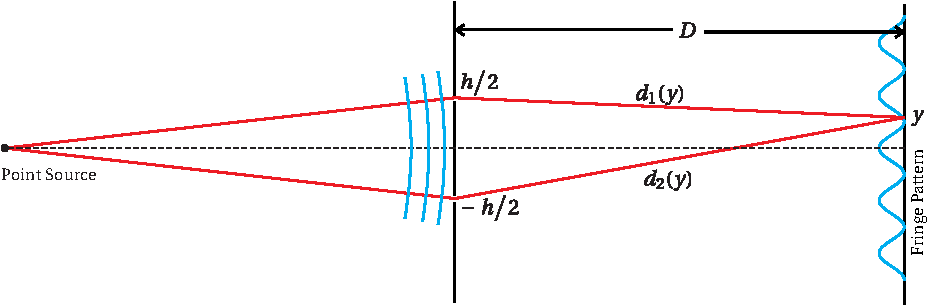
\includegraphics{img/f08Young.pdf}
        \captionof{figure}{Figure caption}
        \label{fig:example} % Unique label used for referencing the figure in-text
    %     %\addcontentsline{toc}{figure}{Figure \ref{fig:placeholder}} % Uncomment to add the figure to the table of contents
    % \end{figure}
    \begin{definition}[big box]
        dsdd
    \end{definition}
\end{fullpage}

\texttt{Figure} is a floating environment and \texttt{minipage} is, unfortunately, not. Therefore, if you put a floating object inside a non-floating minipage, you will get an error.One way is to avoid using figure entirely. This can be done with help of the caption package (with its captionof facility, so that you can have a caption for the figure):
%% solution from https://tex.stackexchange.com/questions/55337/how-to-use-figure-inside-a-minipage
\begin{lstlisting}
    \centering
        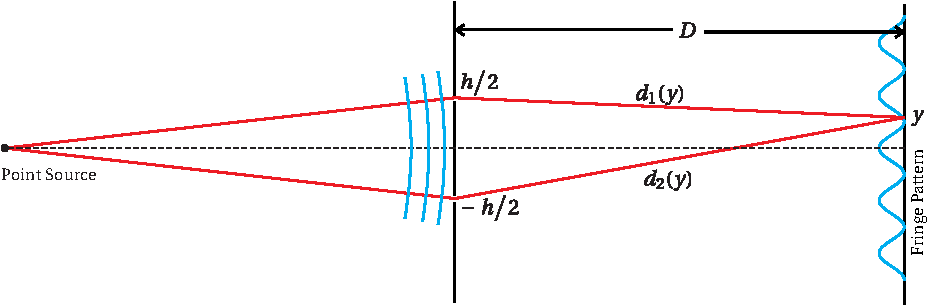
\includegraphics{img/f08Young.pdf}
        \captionof{figure}{Figure caption}
        \label{fig:example} % Unique label used for referencing the figure 
\end{lstlisting}
Table\marginpar{\centering
\begin{tabular}{lll}
\toprule
1 & 1 & 1\\
\midrule
1 & 1 & 0.562 \\
2 & 1 & 0.910 \\
3 & 11 & 0.296 \\
\bottomrule
\end{tabular}
\captionof{table}{Sophisticated margin table}
}The genomes of chimpanzees and humans are 99.9\% identical, yet the differences between the two species are vast. The relatively few differences in genetic endowment must explain \marginpar[right]{dsdsdsdsd}the possession of language by humans, the extraordinary athleticism of chimpanzees, and myriad other differences. Genomic comparison is allowing researchers to identify candidate genes linked to divergences in the developmental programs of humans and the other primates

% \lipsum[2-4]
% Tikz\marginpar{		\begin{center}
%     \begin{tikzpicture}
%         \draw[black,thick] (-1,-1) -- (-.06,-.06);
%         \draw[black,thick] (.06,.06) -- (1,1);
%         \draw[black,thick] (-1,1) -- (1,-1);
%         \filldraw[black] (-1,-1) circle (2pt) node[anchor=north] {2};
%         \filldraw[black] (-1,1) circle (2pt) node[anchor=south] {1};
%         \filldraw[black] (1,-1) circle (2pt) node[anchor=north] {3};
%         \filldraw[black] (1,1) circle (2pt) node[anchor=south] {4};
%     \end{tikzpicture}
% \end{center}
% \captionof{figure}{Marginfigure: Tikz}}



\begin{fullpage}

	\sidebysidecaption{0.555\linewidth}{0.42\linewidth}{%
		\includegraphics[width=1\linewidth]{example-image-a}%
	}{%
	\captionof{figure}{Camera mounted between two
		projections screens. Note that while the view direction can be
		modified, the up vector of the camera is fixed.Camera mounted between two
		projections screens. Note that while the view direction can be
		modified, the up vector of the camera is fixed.}
	  \label{fg:cam-mounting}
	}


\end{fullpage}

\begin{fullpage}

	\sidebysidecaption{0.7\linewidth}{0.25\linewidth}{%
		\includegraphics[width=1\linewidth]{example-image-a}%
	}{%
	\captionof{figure}{Camera mounted between two
		projections screens. Note that while the view direction can be
		modified, the up vector of the camera is fixed.Camera mounted between two
		projections screens. Note that while the view direction can be
		modified, the up vector of the camera is fixed.}
	  \label{fg:cam-mounting}
	}


\end{fullpage}

\begin{fullpage}

	\sidebysidecaption{0.4\linewidth}{0.55\linewidth}{%
		\includegraphics[width=1\linewidth]{example-image-a}%
	}{%
	\captionof{figure}{Camera mounted between two
		projections screens. Note that while the view direction can be
		modified, the up vector of the camera is fixed.Camera mounted between two
		projections screens. Note that while the view direction can be
		modified, the up vector of the camera is fixed.Camera mounted between two
		projections screens. Note that while the view direction can be
		modified, the up vector of the camera is fixed.Camera mounted between two
		projections screens. Note that while the view direction can be
		modified, the up vector of the camera is fixed.}
	}


\end{fullpage}


\begin{fullpage}

	\sidebysidecaption{0.4\linewidth}{0.55\linewidth}{%
	\captionof{figure}{Camera mounted between two
		projections screens. Note that while the view direction can be
		modified, the up vector of the camera is fixed.Camera mounted between two
		projections screens. Note that while the view direction can be
		modified, the up vector of the camera is fixed.Camera mounted between two
		projections screens. Note that while the view direction can be
		modified, the up vector of the camera is fixed.Camera mounted between two
		projections screens. Note that while the view direction can be
		modified, the up vector of the camera is fixed.}
	}{%
    \includegraphics[width=1\linewidth]{example-image-a}%
}


\end{fullpage}


% \bibliography{reference}
% \part{three}

\chapter{Margin Stuff}

Sidenotes are a distinctive feature of all 1.5-column-layout books. 
Indeed, having wide margins means that some material can be displayed 
there. We use margins for all kind of stuff: sidenotes, marginnotes, 
small tables of contents, citations, and, why not?, special boxes and 
environments.

\section{Sidenotes}

Sidenotes are like footnotes, except that they go in the margin, where 
they are more readable. To insert a sidenote, just use the command 
\Command{sidenote\{Text of the note\}}. You can specify a 
mark\sidenote[O]{This sidenote has a special mark, a big O!} with \\ 
\Command{sidenote[mark]\{Text\}}, but you can also specify an offset, 
which moves the sidenote upwards or downwards, so that the full syntax is:

\begin{lstlisting}
\sidenote[mark][offset]{Text}
\end{lstlisting}

If you use an offset, you always have to add the brackets for the mark, 
but they can be empty.\sn{If you want to know more about the usage 
of the \Command{sidenote} command, read the documentation of the 
\Package{sidenotes} package.}

In \Class{subook} we copied a feature from the \Package{snotez} 
package: the possibility to specify a multiple of \Command{baselineskip} 
as an offset. For example, if you want to enter a sidenote with the 
normal mark and move it upwards one line, type:

\begin{lstlisting}
\sidenote[][*-1]{Text of the sidenote.}
\end{lstlisting}

As we said, sidenotes are handled through the \Package{sidenotes} 
package, which in turn relies on the \Package{marginnote} package.

\section{Marginnotes}

This command is very similar to the previous one. You can create a 
marginnote with 

\Command{marginnote[offset]\{Text\}}

,where the offset 
argument can be left out, or it can be a multiple of \mn{While the command for margin 
notes comes from the \Package{marginnote} package, it has been redefined 
in order to change the position of the optional offset argument, which 
now precedes the text of the note, whereas in the original version it 
was at the end. We have also added the possibility to use a multiple of 
\Command{baselineskip} as offset. These things were made only to make 
everything more consistent, so that you have to remember less things! }


\begin{lstlisting}
\marginnote[-12pt]{Text} or \marginnote[*-3]{Text}
\end{lstlisting}

Since \Package{sidenotes} uses \Package{marginnote}, 
what we said for marginnotes is also valid for sidenotes. Side- and 
margin- notes are shifted slightly upwards 

(\Command{renewcommand\{\textbackslash marginnotevadjust\}\{3pt\}}) 

in 
order to align them to the bottom of the line of text where the note is 
issued. Importantly, both sidenotes and marginnotes are defined as 
floating if the optional argument ( the vertical offset) is left 
blank, but if the offset is specified they are not floating. Recall that 
floats cannot be nested, so in some rare cases you may encounter errors 
about lost floats; in those cases, remember that sidenotes and 
marginnotes are floats. To solve the problem, it may be possible to 
transform them into non-floating elements by specifying an offset of 
0pt.

\section{Why use both \Package{marginnotes} and \Package{sidenotes}?}

Quite simply, \Package{marginnotes} overlap each other if they are too close. This means that figures, and tables can overlap by just using \Package{marginnotes}. 
This is why \Package{sidenotes} is so useful as it not only numbers all side notes, but also dynamically aligns all side notes, figures, and tables.

So clearly, \Package{sidenotes} must be better right? 
There are a few places where \Package{sidenotes} fails too however. 
For instance, \Package{sidenotes} cannot be used in equations, \Package{multicols}, and with the \Package{tcolorbox} for more details.environment. 
As the majority of the special environments from \Package{amsthm} are modified to use \Package{tcolorbox}, \Package{marginnotes} becomes an essential part of \Package{NotesTeX}.

The implementation of each of these is as follows.
\begin{enumerate}
    \item \texttt{Marginnote:} This is how a \texttt{$\backslash$marginnote\{...\}} behaves.\marginnote{Not numbered, 10pt.}
    \item \texttt{Mn:} This is how a \texttt{$\backslash$mn\{...\}} behaves.\mn{Numbered, footnotesize.}
    \item \texttt{Sidenote:} This is how a \texttt{$\backslash$sidenote\{...\}} behaves.\sidenote{Numbered, 10pt.}
    \item \texttt{Sn:} This is how a \texttt{$\backslash$sn\{...\}} behaves.\sn{Numbered, footnotesize.}
    \item \texttt{Marginfigure:} This environment requires the \texttt{$\backslash$begin\{marginfigure\}} {$\cdots$}\newline\texttt{$\backslash$end\{marginfigure\}} enclosings. The \texttt{caption} package is needed to caption the figure.
    \begin{marginfigure}
    \begin{center}
        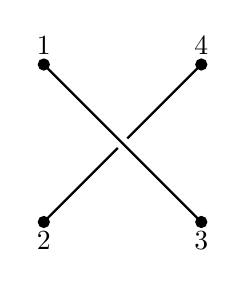
\begin{tikzpicture}
            \draw[black,thick] (-1,-1) -- (-.06,-.06);
            \draw[black,thick] (.06,.06) -- (1,1);
            \draw[black,thick] (-1,1) -- (1,-1);
            \filldraw[black] (-1,-1) circle (2pt) node[anchor=north] {2};
            \filldraw[black] (-1,1) circle (2pt) node[anchor=south] {1};
            \filldraw[black] (1,-1) circle (2pt) node[anchor=north] {3};
            \filldraw[black] (1,1) circle (2pt) node[anchor=south] {4};
        \end{tikzpicture}
    \end{center}
    \captionof{figure}{Marginfigure: Tikz}
    \end{marginfigure}%
    \item \texttt{Margintable:} This environment requires the \texttt{$\backslash$begin\{margintable\}} {$\cdots$}\newline\texttt{$\backslash$end\{margintable\}} enclosings. A table package, such as \texttt{tabular}, \texttt{tabulary}, \texttt{tabu}, or \texttt{tabularx} is required. The \texttt{caption} package is needed to caption the table.
    \begin{margintable}
        \vspace{.1in}
        \begin{tabularx}{\marginparwidth}{|X|X|}
        \hline
        \textit{NotesTeX} & \textbf{rocks!}\\
        \hline
        \end{tabularx}
        \caption{Margintable}
    \end{margintable}
\end{enumerate}


\part{Biology notes}
\chapter[DNA, Chromosomes, and Genomes]{DNA, Chromosomes, \protect\\and Genomes}\labch{re}
The documents of biology, chemistry and other disciplines are characterized by more legends and noun explanations, and less formulas. Here we have created an command \Package{sidebysidecaption} to freely adjust the size of legends and figures.We use a portion of Chapter 4 of \citetitle{thecell}\sidecite{thecell}
 for our template presentation.



\section{The Structure of DNA Provides a mechanism for Heredity}\labsec{structure}

The discovery of the structure of DNA immediately suggested answers to the two
most fundamental questions about heredity. First, how could the information to
specify an organism be carried in a chemical form? And second, how could this
information be duplicated and copied from generation to generation?

The answer to the frst question came from the realization that DNA is a linear
polymer of four different kinds of monomer, strung out in a defned sequence like
the letters of a document written in an alphabetic script.

The answer to the second question came from the double-stranded nature of
the structure: because each strand of DNA contains a sequence of nucleotides
that is exactly complementary to the nucleotide sequence of its partner strand,
each strand can act as a \key{template}, or mold, for the synthesis of a new complementary strand. In other words, if we designate the two DNA strands as S and Sʹ, strand 

\begin{fullpage}

	\sidebysidecaption{0.5\linewidth}{0.45\linewidth}{%
		\includegraphics[width=1\linewidth]{img/double_helix.png}%
	}{%
	\captionof{figure}{The DNA double helix.
    (A) A space-flling model of 1.5 turns of
    the DNA double helix. Each turn of DNA is
    made up of 10.4 nucleotide pairs, and the
    center-to-center distance between adjacent
    nucleotide pairs is 0.34 nm. The coiling of
    the two strands around each other creates
    two grooves in the double helix: the wider
    groove is called the major groove, and the
    smaller the minor groove, as indicated.
    (b) A short section of the double helix
    viewed from its side, showing four base
    pairs. The nucleotides are linked together
    covalently by phosphodiester bonds that
    join the 3ʹ-hydroxyl (–OH) group of one
    sugar to the 5ʹ-hydroxyl group of the next
    sugar. Thus, each polynucleotide strand
    has a chemical polarity; that is, its two
    ends are chemically different. The 5ʹ end
    of the DNA polymer is by convention often
    illustrated carrying a phosphate group,
    while the 3ʹ end is shown with a hydroxyl}
    }
\end{fullpage}

S can serve as a template for making a new strand Sʹ, while strand Sʹ can serve as a
template for making a new strand S (\vreffig{template}). Thus, the genetic information in
DNA can be 
accurately copied by the beautifully simple process in which strand
S separates from strand Sʹ, and each separated strand then serves as a template
for the production of a new complementary partner strand that is identical to its
former partner.

\begin{fullpage}

	\sidebysidecaption{0.5\linewidth}{0.45\linewidth}{%
		\includegraphics[width=1\linewidth]{img/template.png}%
        \labfig{template}}{%
	\captionof{figure}{DNA as a template for its
    own duplication. because the nucleotide
    A successfully pairs only with T, and g
    pairs with C, each strand of DNA can act
    as a template to specify the sequence of
    nucleotides in its complementary strand.
    In this way, double-helical DNA can be
    copied precisely, with each parental DNA
    helix producing two identical daughter DNA
    helices.}
    }
    
\end{fullpage}

The ability of each strand of a DNA molecule to act as a template for producing
a complementary strand enables a cell to copy, or replicate, its genome before
passing it on to its descendants. We shall describe the elegant machinery that the
cell uses to perform this task in Chapter 5.

Organisms differ from one another because their respective DNA molecules
have different nucleotide sequences and, consequently, carry different biological
messages. But how is the nucleotide alphabet used to make messages, and what do they spell out?

As discussed above, it was known well before the structure of DNA was determined that genes contain the instructions for producing proteins. If genes are made of DNA, the DNA must therefore somehow encode proteins (\vreffig{relation})\marginpar{
    \centering
    \includegraphics[width=0.4\textwidth]{img/relation.png}
    \captionof{figure}{The relationship between
    genetic information carried in DNA and
    proteins.}\labfig{relation}}.

As discussed in Chapter 3, the properties of a protein, which are responsible for its
biological function, are determined by its three-dimensional structure. Tis structure is determined in turn by the linear sequence of the amino acids of which it is
composed. The linear sequence of nucleotides in a gene must therefore somehow
spell out the linear sequence of amino acids in a protein. The exact correspondence between the four-letter nucleotide alphabet of DNA and the twenty-letter
amino acid alphabet of proteins—the genetic code—is not at all obvious from the
DNA structure, and it took over a decade after the discovery of the double helix
before it was worked out. In Chapter 6, we will describe this code in detail in the
course of elaborating the process of gene expression, through which a cell converts
the nucleotide sequence of a gene frst into the nucleotide sequence of an RNA
molecule, and then into the amino acid sequence of a protein.



\part{Machine Learning Notes}
\include{chapters/probility.tex}

\pagestyle{empty}

\printbibliography[heading=bibliography,title=Bibliography]

\stepcounter{part}
\appendix
\include{chapters/appendix.tex}
\blinddocument



% \chapter{Margin Stuff}

Sidenotes are a distinctive feature of all 1.5-column-layout books. 
Indeed, having wide margins means that some material can be displayed 
there. We use margins for all kind of stuff: sidenotes, marginnotes, 
small tables of contents, citations, and, why not?, special boxes and 
environments.

\section{Sidenotes}

Sidenotes are like footnotes, except that they go in the margin, where 
they are more readable. To insert a sidenote, just use the command 
\Command{sidenote\{Text of the note\}}. You can specify a 
mark\sidenote[O]{This sidenote has a special mark, a big O!} with \\ 
\Command{sidenote[mark]\{Text\}}, but you can also specify an offset, 
which moves the sidenote upwards or downwards, so that the full syntax is:

\begin{lstlisting}
\sidenote[mark][offset]{Text}
\end{lstlisting}

If you use an offset, you always have to add the brackets for the mark, 
but they can be empty.\sn{If you want to know more about the usage 
of the \Command{sidenote} command, read the documentation of the 
\Package{sidenotes} package.}

In \Class{subook} we copied a feature from the \Package{snotez} 
package: the possibility to specify a multiple of \Command{baselineskip} 
as an offset. For example, if you want to enter a sidenote with the 
normal mark and move it upwards one line, type:

\begin{lstlisting}
\sidenote[][*-1]{Text of the sidenote.}
\end{lstlisting}

As we said, sidenotes are handled through the \Package{sidenotes} 
package, which in turn relies on the \Package{marginnote} package.

\section{Marginnotes}

This command is very similar to the previous one. You can create a 
marginnote with 

\Command{marginnote[offset]\{Text\}}

,where the offset 
argument can be left out, or it can be a multiple of \mn{While the command for margin 
notes comes from the \Package{marginnote} package, it has been redefined 
in order to change the position of the optional offset argument, which 
now precedes the text of the note, whereas in the original version it 
was at the end. We have also added the possibility to use a multiple of 
\Command{baselineskip} as offset. These things were made only to make 
everything more consistent, so that you have to remember less things! }


\begin{lstlisting}
\marginnote[-12pt]{Text} or \marginnote[*-3]{Text}
\end{lstlisting}

Since \Package{sidenotes} uses \Package{marginnote}, 
what we said for marginnotes is also valid for sidenotes. Side- and 
margin- notes are shifted slightly upwards 

(\Command{renewcommand\{\textbackslash marginnotevadjust\}\{3pt\}}) 

in 
order to align them to the bottom of the line of text where the note is 
issued. Importantly, both sidenotes and marginnotes are defined as 
floating if the optional argument ( the vertical offset) is left 
blank, but if the offset is specified they are not floating. Recall that 
floats cannot be nested, so in some rare cases you may encounter errors 
about lost floats; in those cases, remember that sidenotes and 
marginnotes are floats. To solve the problem, it may be possible to 
transform them into non-floating elements by specifying an offset of 
0pt.

\section{Why use both \Package{marginnotes} and \Package{sidenotes}?}

Quite simply, \Package{marginnotes} overlap each other if they are too close. This means that figures, and tables can overlap by just using \Package{marginnotes}. 
This is why \Package{sidenotes} is so useful as it not only numbers all side notes, but also dynamically aligns all side notes, figures, and tables.

So clearly, \Package{sidenotes} must be better right? 
There are a few places where \Package{sidenotes} fails too however. 
For instance, \Package{sidenotes} cannot be used in equations, \Package{multicols}, and with the \Package{tcolorbox} for more details.environment. 
As the majority of the special environments from \Package{amsthm} are modified to use \Package{tcolorbox}, \Package{marginnotes} becomes an essential part of \Package{NotesTeX}.

The implementation of each of these is as follows.
\begin{enumerate}
    \item \texttt{Marginnote:} This is how a \texttt{$\backslash$marginnote\{...\}} behaves.\marginnote{Not numbered, 10pt.}
    \item \texttt{Mn:} This is how a \texttt{$\backslash$mn\{...\}} behaves.\mn{Numbered, footnotesize.}
    \item \texttt{Sidenote:} This is how a \texttt{$\backslash$sidenote\{...\}} behaves.\sidenote{Numbered, 10pt.}
    \item \texttt{Sn:} This is how a \texttt{$\backslash$sn\{...\}} behaves.\sn{Numbered, footnotesize.}
    \item \texttt{Marginfigure:} This environment requires the \texttt{$\backslash$begin\{marginfigure\}} {$\cdots$}\newline\texttt{$\backslash$end\{marginfigure\}} enclosings. The \texttt{caption} package is needed to caption the figure.
    \begin{marginfigure}
    \begin{center}
        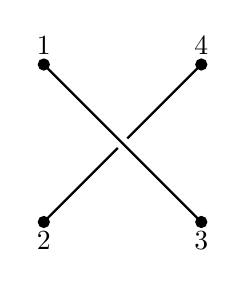
\begin{tikzpicture}
            \draw[black,thick] (-1,-1) -- (-.06,-.06);
            \draw[black,thick] (.06,.06) -- (1,1);
            \draw[black,thick] (-1,1) -- (1,-1);
            \filldraw[black] (-1,-1) circle (2pt) node[anchor=north] {2};
            \filldraw[black] (-1,1) circle (2pt) node[anchor=south] {1};
            \filldraw[black] (1,-1) circle (2pt) node[anchor=north] {3};
            \filldraw[black] (1,1) circle (2pt) node[anchor=south] {4};
        \end{tikzpicture}
    \end{center}
    \captionof{figure}{Marginfigure: Tikz}
    \end{marginfigure}%
    \item \texttt{Margintable:} This environment requires the \texttt{$\backslash$begin\{margintable\}} {$\cdots$}\newline\texttt{$\backslash$end\{margintable\}} enclosings. A table package, such as \texttt{tabular}, \texttt{tabulary}, \texttt{tabu}, or \texttt{tabularx} is required. The \texttt{caption} package is needed to caption the table.
    \begin{margintable}
        \vspace{.1in}
        \begin{tabularx}{\marginparwidth}{|X|X|}
        \hline
        \textit{NotesTeX} & \textbf{rocks!}\\
        \hline
        \end{tabularx}
        \caption{Margintable}
    \end{margintable}
\end{enumerate}

% \include{CN_Chapters/page.tex}
\end{document}